\documentclass[usletter]{article} 
\usepackage[margin=1in]{geometry} 
\usepackage{graphicx} 
\usepackage{hyperref} 
\usepackage{fancyhdr} 

\pagestyle{fancy} 
\fancyhf{} 
\rhead{BEACON Surveyer User Guide v0.1} 
\lhead{Pg. \thepage} 


\title{BEACON Surveyer User Guide} 
\author{Cosmin Deaconu
\\ \href{mailto:cozzyd@kicp.uchicago.edu}{cozzyd@kicp.uchicago.edu} 
}


\begin{document} 

\maketitle

\tableofcontents

\section{Introduction} 

This document describes the theory and operation of the BEACON antenna surveying system.
This system is a low-cost alternative to a commercial real-time kinematic (RTK)
surveying system.  

The purpose of the system is to precisely measure the three-dimensional
positions  of a set of points relative to a common origin. In particular, for
BEACON, we need to know the relative position sof the antenna in
three-dimensions to a few centimeters in order to make measurements.  The
system uses two Global Navigation Satellite Service (GNSS, although GPS is used mostly interchangeably in this document) units that can talk to each other wirelesslyand a laptop
for logging the data. 

For any questions, please contact Cosmin via e-mail, or, if urgent, by mobile phone (775.846.9105).


\section{How it works} 


\subsection{Theory of Operation} 

\textit{You can skip this section if you don't care :), but do read the next subsection!} 

GNSS systems work by measuring relative time delays of radio signals from
various satellite constellations. The most well-known is the Global Positioning
System (GPS) commissioned by the United States, but nowadays there are several
other constellations (the Russioan GLONASS, European Galileo, and Chinese
Beidou) that can be used in concert. Still, in this document GPS and GNSS will 

Normally, at least with the unrestricted civilian bands, one can obtain
position accuracy of around 1 meter with a GNSS receiver. The precision is limited
due to fluctuations in the radio transmission properties of the part of the
Earth's atmosphere (the ionosphere), that cannot be perfectly corrected for. 


However, if you have two receivers that are relatively close together, they
experience almost exactly the same fluctuations for every satellite. This means
that if you only care about the relative position of the two units, you can
essentially subtract out the atmospheric fluctuations, giving allowing
measurement of relative positions to an accuracy of a few cm under good
conditions. A system set up to do this is genrally called a Real-Time Kinematic
(RTK) system. 

Moreover, there are multiple frequencies available with GNSS satellites, and
if you have a receiver that can receive multiple frequencies (a ``dual-band"
receiver), for technical reasons, it is possible to use the additional
information to find a solution to the distance between the receivers more
quickly.

\subsection{ Overview of the BEACON survey system} 

The BEACON survey system consists of two dual-band GPS receiver development
boards (u-blox C099-F9P boards, if you care), which have been  configured to talk to each other via WiFi.

The two boards are configured differently, and appropriately labeled. One is
the \textbf{Base}.  The Base is configured a WiFi router, and can transmit the information
necessary to make corrections to any clients over WiFi. Normally the base is stationary with ``known" coordinates so that the rover's absolute position may be determined, but since we only care about the relative coordinates, the Base is configured as a ``moving base"  so it does not matter if the base is stationary or the Rover is. 

The other board is the \textbf{Rover}, which is configured to connect to the
Base automatically over WiFi so that it can receive the atmospheric corrections
necessary. Once it starts receiving enough connections, it can calculate its 3D
coordinates relative to the Base. By connecting a laptop to the Rover via USB,
we can read out this 3D relative position. To facilitate that, a custom
graphical user interface has been developed. 

Note that when we talk about the relative difference between the two boards, we
really mean the relative distance between the GPS antennas. It is the location
of the antenna that is actually being measured, not the board itself! 



\section{System Contents and Assembly}  

This section describes the components of the BEACON survey system and how to put them together. A specific order of operation will be given in the Operation section. 

\subsection{Contents} 

You should have received two boxes (with u-blox packaging) as well as a laptop  (a relatively old IBM Thinkpad) and a power adapter. 

Inside each of the boxes, you should have: 

\begin{itemize} 
\item A GPS receiver, in a 3-D printed enclosure, labeled ROVER or BASE (this will probably be in an anti-static bag) 
\item A microusb cable
\item A USB-to-DC power cable 
\item A GPS Antenna (with a longish RG174 cable with SMA connector) 
\item A metal disc (this is the GPS antenna backplane) 
\item A WiFi antenna 
\end{itemize} 


\subsection{The receiver units} 

The base and rover receivers both come in a custom 3-D printed enclosure and
are labeled accordingly. They are not interchangeable as the firmware is
configured differently, although all other components are interchangeable.  

\begin{center} 
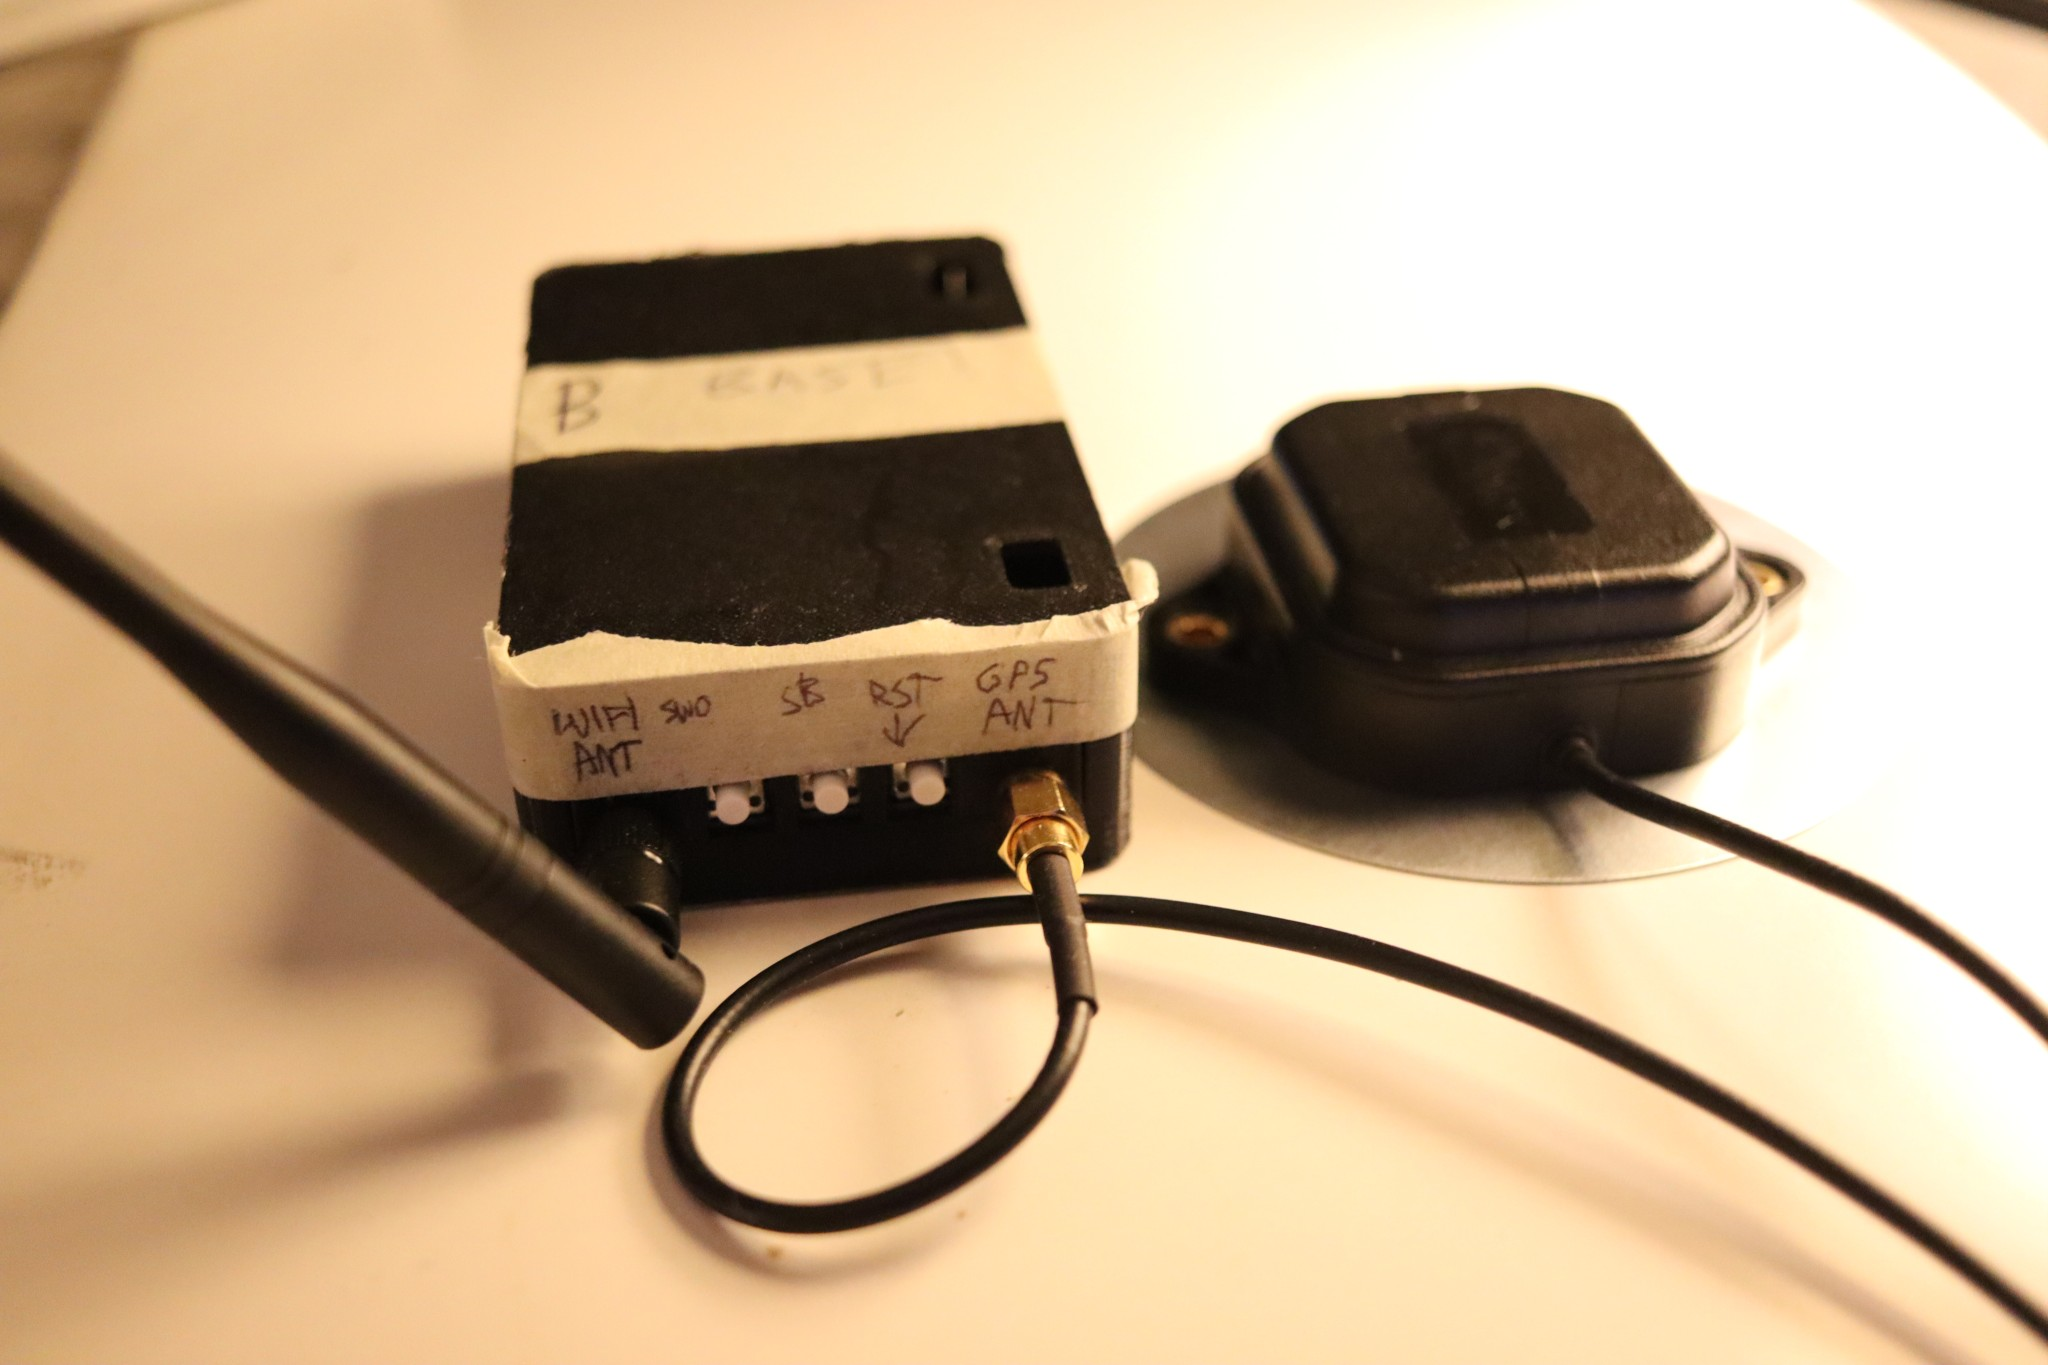
\includegraphics[width=4in]{receiver-front} 
\end{center} 

Each unit has two RF connectors (SMA-type). One is for the WiFi antenna, the
other is for the GNSS (labeled GPS on the uunit) antenna. \textbf{The GPS Antenna is active so it should be
plugged in while the sytem is off. Turning the system on without the GPS
antenna plugged in could result in a shock and/or damage to the system.}. 

There are three buttons on the front of the receiver. The only one you are
likely to use is the Reset (RST) button, which resets the unit.
\textbf{Holding the button labelled SW0 for 3 seconds will clear the firmware
of the receivers. Don't do that since we don't yet have an automatic way of
configuring the receivers and doing it right now  is an error-prone manual
process!!!} 

\begin{center} 
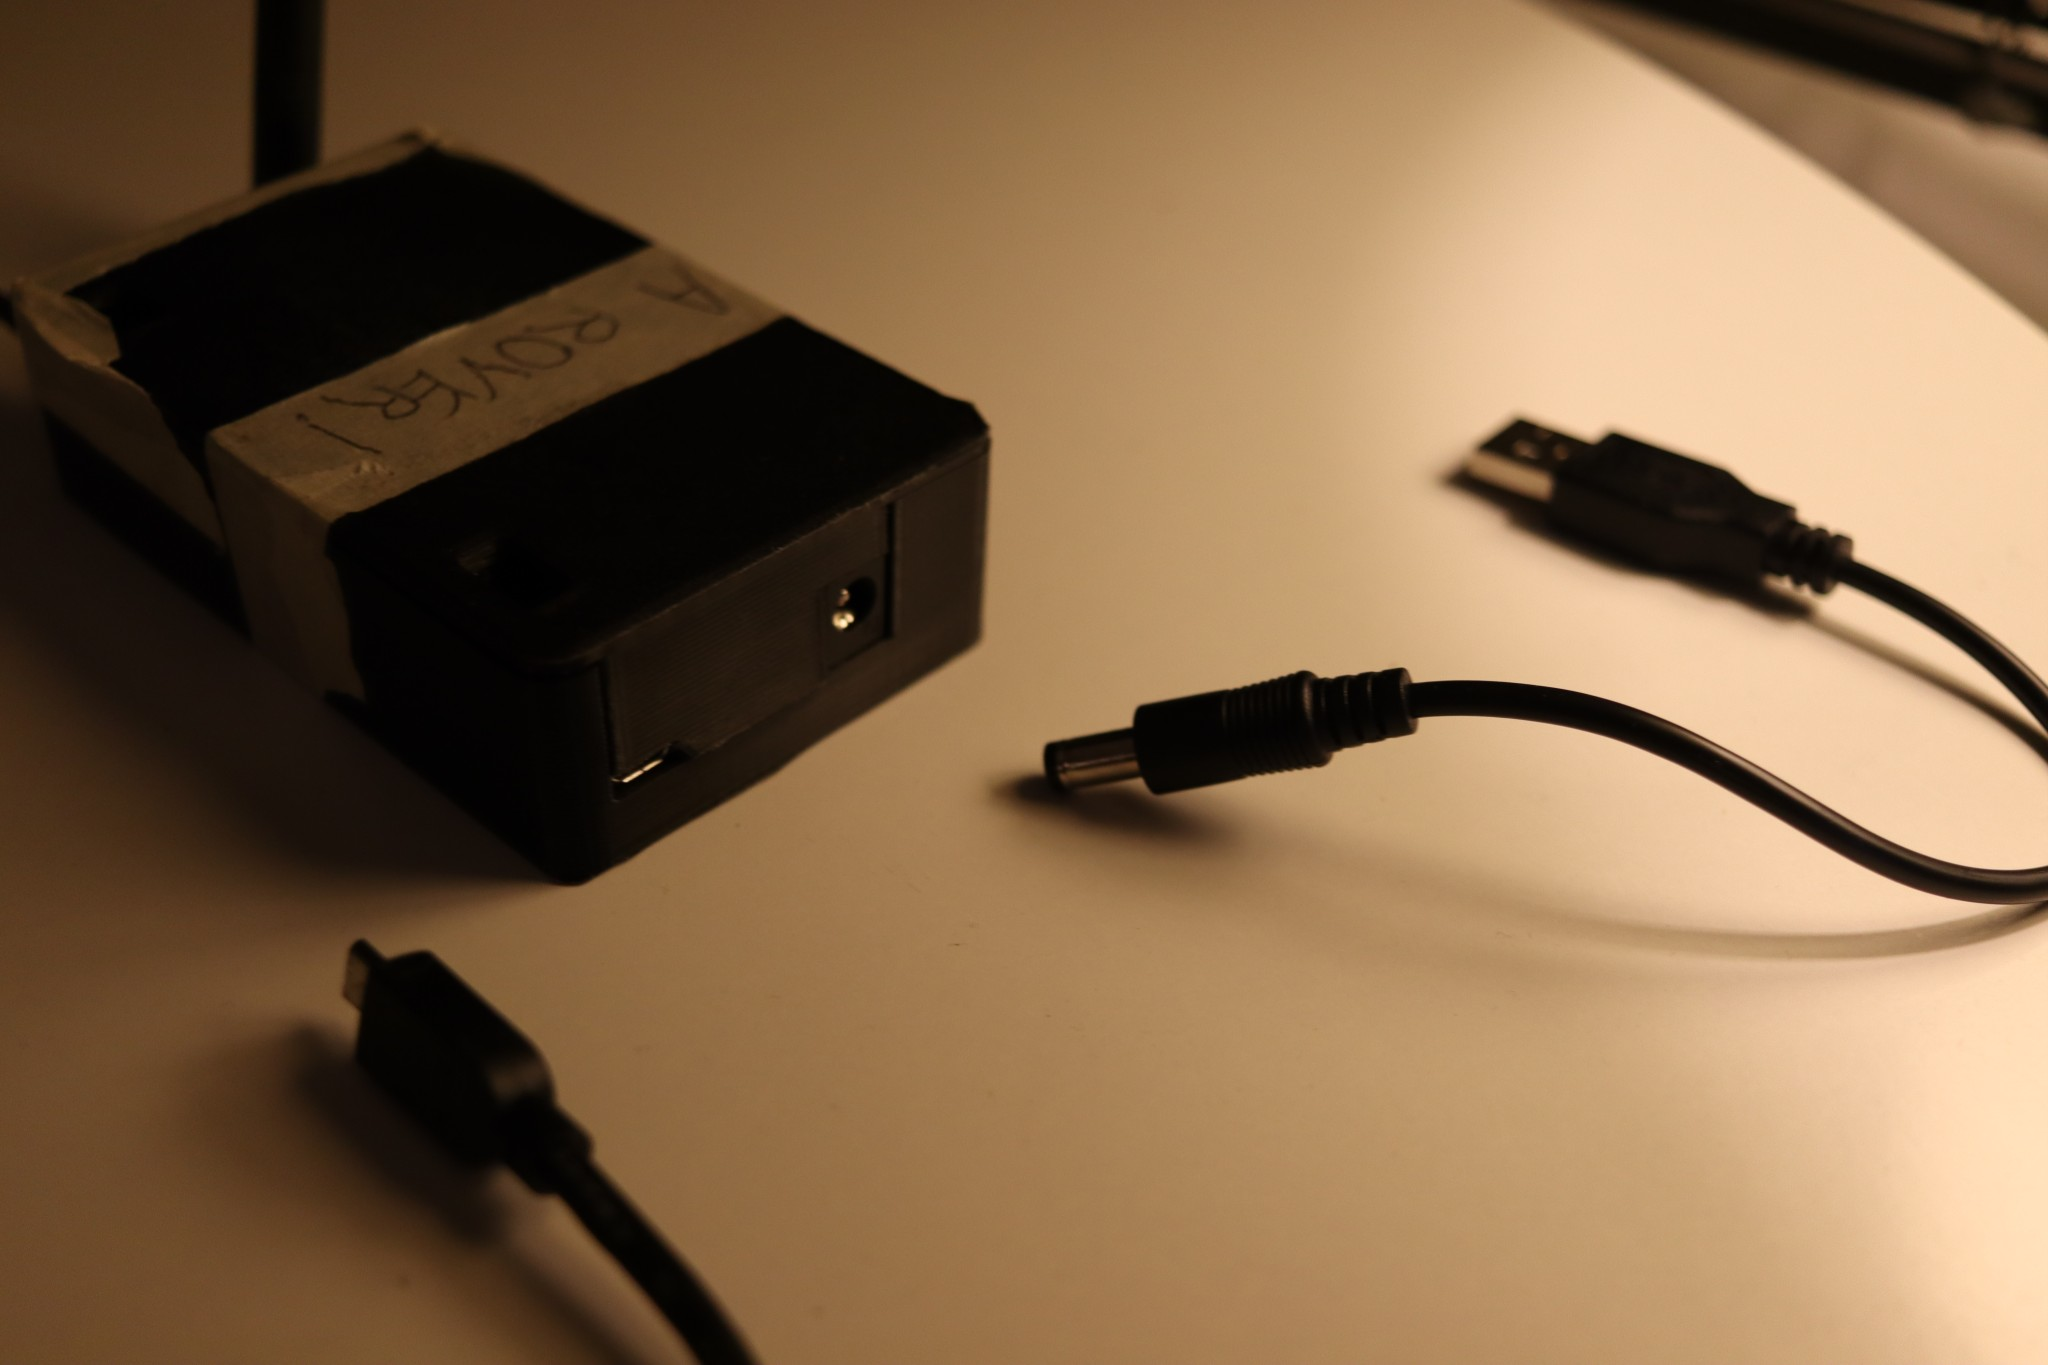
\includegraphics[width=4in]{receiver-back} 
\end{center} 

On the back is a microusb port and a DC power port. The boards can be powered
over microusb if they are plugged into a computer (a microusb cable is
provided) , but, at least for me, using e.g. a USB battery bank, the microusb
connector didn't work for power and I had to power it through the DC port via
the USB-to-DC cable. \textbf{You probably don't want to plug in both the DC
cable and the micro-usb cable}. 

Each unit has two holes at the top so you can see the LED's on the board. There are three LED's that are interesting. 
\begin{enumerate} 
  \item Near the GPS connector, there is the LED for the radio unit. This will be green when the unit is on and purple when the Base and Rover are properly connected to each other via WiFi. The purple LED will flash when the Base is sending data to the Rover (this flashing is intermittent and may not be perceptible). 
  \item Near the microusb port, there is a blue LED for the GPS. If solid, it means that the GPS has turned on. If outside with a good view to the sky, it should soon flashing once a second,  which means the GPS has got a lock (i.e. it knows where it is). It should start flashing. 
  \item Next to the GPS LED is a yellow/green LED for the RTK status. If flashing, it's starting to do an RTK calcualtion. If solid it means that we have an RTK solution (this is the dream!)
\end{enumerate}

There is one more LED that is visible but it won't turn on (it's used as a Geofencing indicator). 

\subsection{The GNSS Antenna} 

The GPS antenna is meant to be used with a metal backplane. That is why it comes with a metal disc, which will magnetically attach to the bottom of the antenna. The antenna is meant to be horizontal, with the disc (or another metal backplane) below in the orientation shown here: 

\begin{center} 
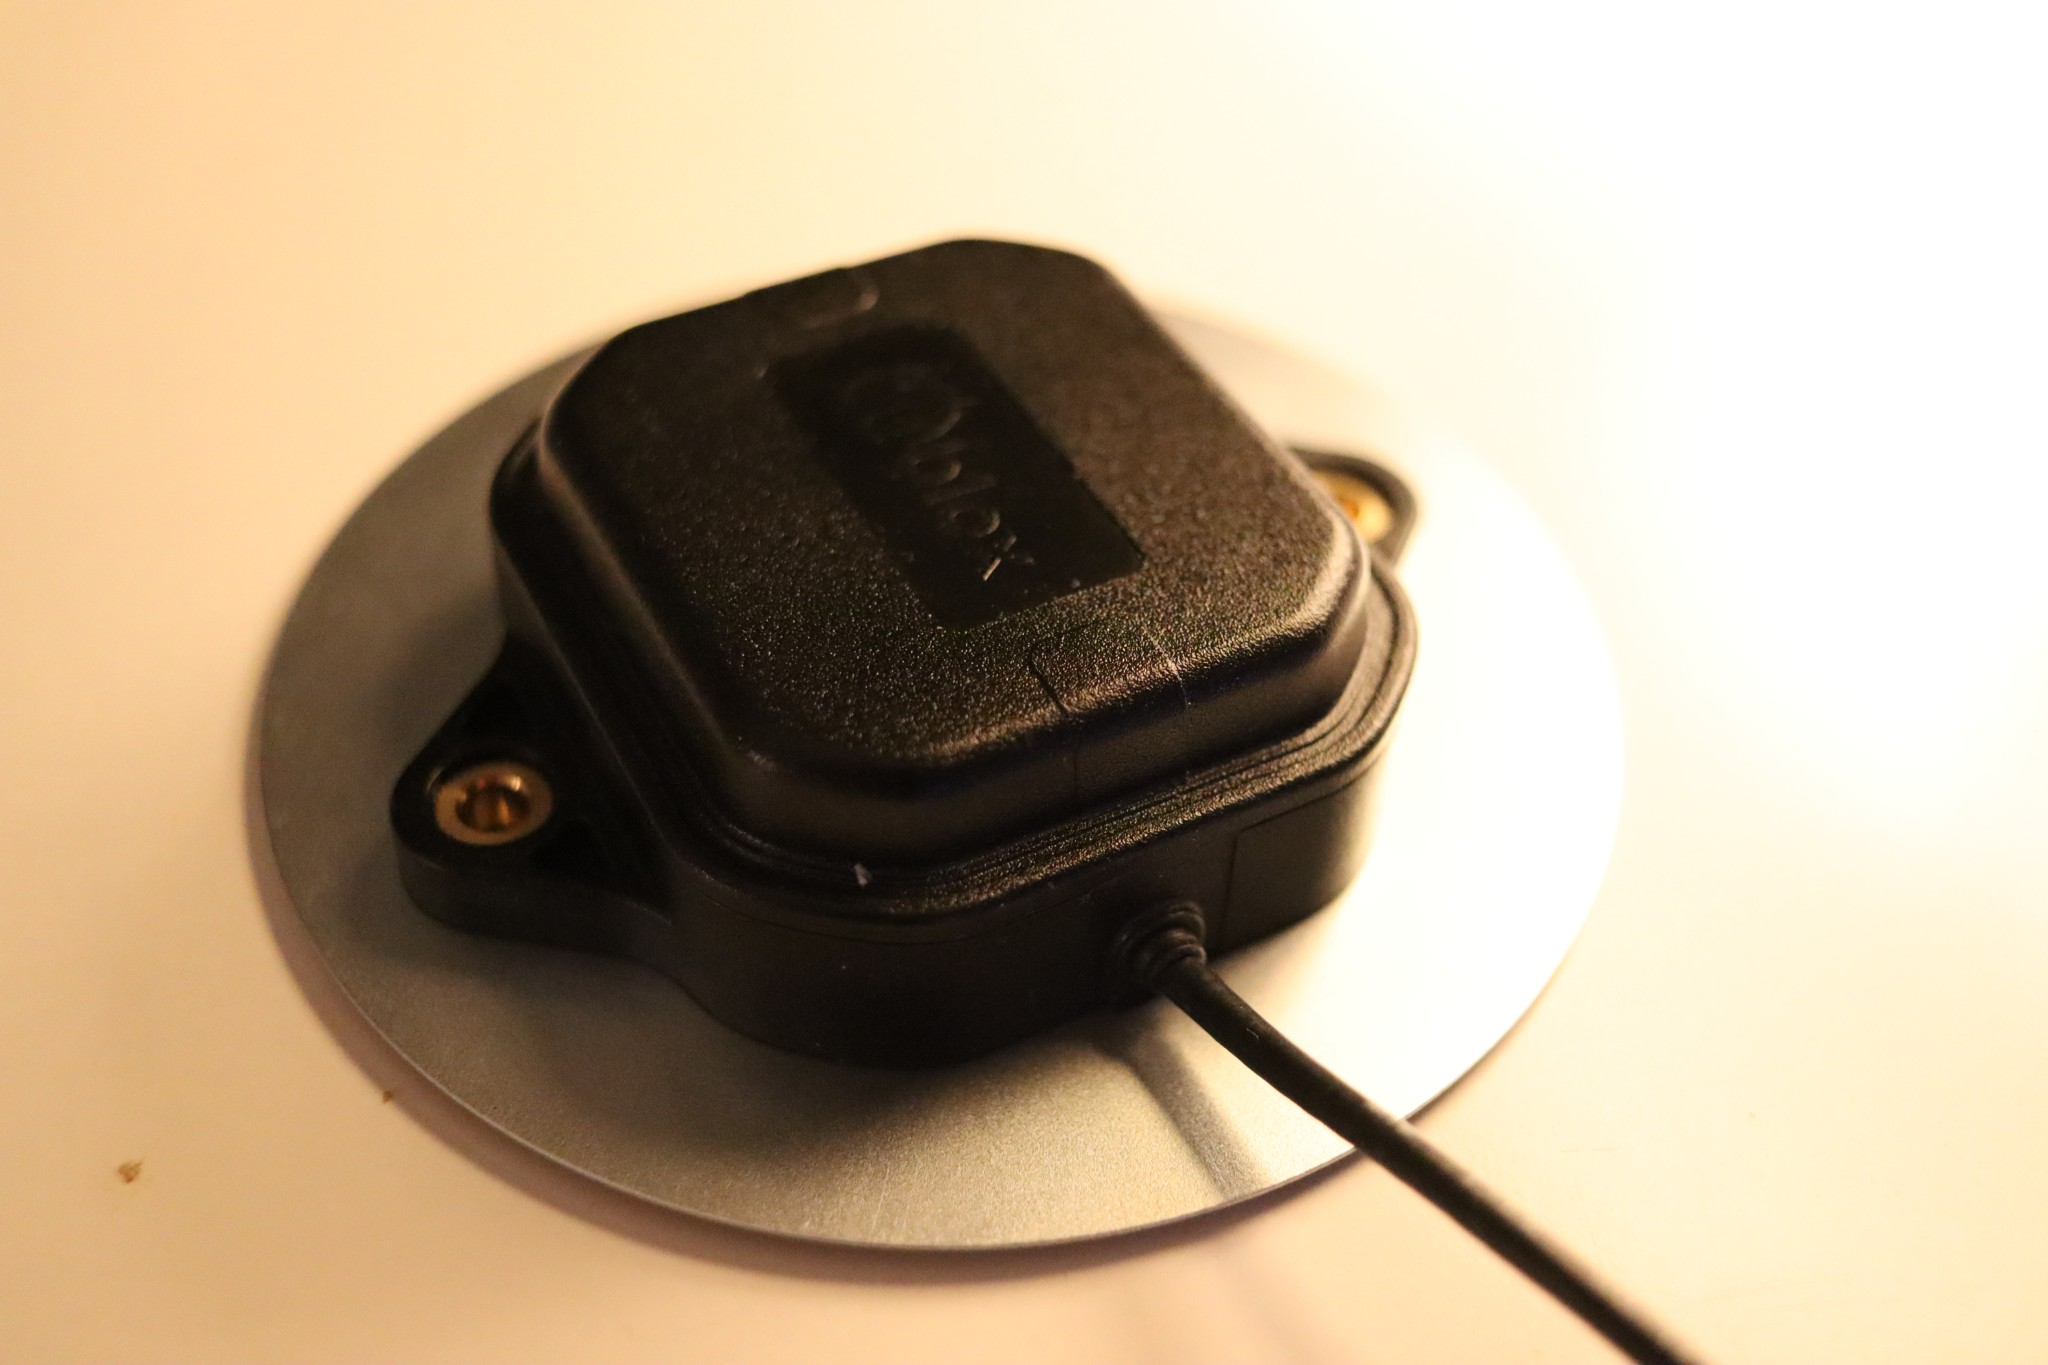
\includegraphics[width=4in]{gps-antenna} 
\end{center}

\subsection{The Laptop} 

A now-ancient small-but-bricky laptop is provided. This laptop is slow and clunky and has a hard drive (not a solid-state drive!) that hopefully won't fail at altitude. It has several accounts on it, with several sticky notes with credentials. \textbf{Use the survey account, with the password on the sticky note, as that has the software for reading out the Rover available}. The battery works fairly well and should last at least several hours. 

Eventually, the Rover will be plugged into the laptop via USB. On the top left of the desktop is a shortcut to launch the Rover data logger program. Usage of this program is described in the Operation section. 

\section{Operation} 

This section describes the recommended method to perform the measurement. Please read this at least once before actually doing it! 

\subsection{Set up the base receiver} 

If you haven't already, plug in the GPS antenna and WiFi antenna into the Base
unit. Even though this is called the base, since it does not need to be
connected to a laptop for readout, it is probably easier to move the ``base" around and
keep the ``rover" stationary!  Either is fine, but I'm guessing it will be easier not to have tomovemvoe the laptop. 

Either way, the base should be turned on first because
the Rover must connect to the Base (of course, after powering on, you can
always reset the two in sequence if they get confused or you powered them on in
the wrong order). 

I recommend using a USB battery bank with the USB to DC connector to power the
base. Any decent battery bank should power the unit for many hours. I do not
recommend plugging it via microusb into the same laptop as the Rover because then it will
make it more difficult to figure out which receiver you talking to with the
laptop. 

The blue LED should start blinking once a second relatively soon after turning it on outside. 


\subsection{Set up the rover receiver} 

If you haven't aready, plug in the GPS antenna and WiFi antenna into the rover
unit. Unlike the base, the Rover must be plugged into the laptop via microusb
(which will also power it on). The rover is more likely to properly connect to
the base if it's turned on afterwards (because that's when it will definitely
be trying to make a WiFi connection). If you turned on the rover before the
base, just reset the rover. 

Either the rover or base must remain stationary throughout the measurements, but as mentioned above, because the
rover has to be connected to the laptop, it's easier if the rover is
stationary.  This means \textbf{don't move the Rover antenna once you've started doing measurements!} 

Once the Rover connects to the Base, the purple radio LED will turn on for
both. The Rover's blue LED should start blinking soon after it's turned on and
the yellow/green LED should hopefully start blinking and then turning solid
soon thereafter. If the yelow/green LED doesn't turn on, that means we're not
getting an RTK solution and we need to figure out why. 

\subsection{Reading out data from the rover} 

Start the GUI program (upper left corner of the desktop). A command window will pop up and a few seconds a gui will pop up. An annotated version is below:

\begin{center} 
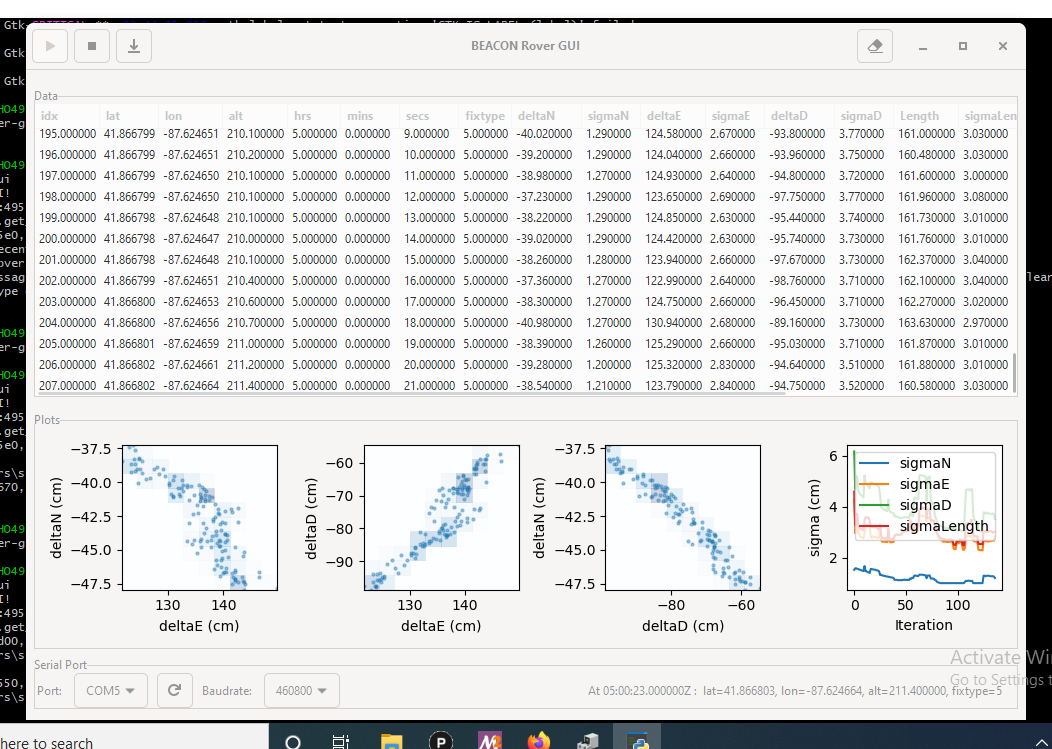
\includegraphics[width=4in]{gui} 
\end{center} 

On the top are the controls to start taking data, stop taking data, save the data, or clear all the data. Enter toggles betwen starting/stopping data and ctrl-S and ctrl-L are shortcuts for saving data and clearing data, respectively. 
On the bottom is  the configuration for the serial port and the status bar. Unfortunately, the GPS receiver actually presents 3 different serial ports to the laptop, and only two of the three can be used to communicate with it. Because the names are not consistent, sometimes we get it wrong. If you start taking data but the status bar says something about no data being received, either the blue light isn't flashing on the Rover (unlikely if you've waited more than a few seconds and are outside) or the wrong serial port is selected. Stop taking data and try a different one. 
A fool-proof method to get the serial port right is presented in the troubleshooting section.

In the middle is a table of collected relative position data and some diagnostic plots. When there is an RTK solution and we are taking data, a new row should appear about once a second. If we have a good solution, then the values for delta N (/orth), delta E (East) and delta D (Down?) should cluster and sigma N/E/D should be relatively small (those are all plotted). If it's jumping around a lot, we probably don't have a good solution yet. 

\subsection{Measuring the positions of the BEACON antennas} 

Using this system, it is possible to measure the relative positions of the BEACON antenna masts relative to a fixed point. To do this, place the base antenna at the base of each mast, let it get a fix, then go to the laptop, clear any existing data and record data until we have enough readings that seem reasonable, meaning  that the points start getting clustered together and the errors (sigmas) on the distances are small. Oncce we have enough good points, save (with the mast number), and move the base antenna to the next mast and repeat. Make sure you leave the rover antenna fixed for the entire duration so that all measurements have the same reference point. 

\section{Troubleshooting} 

\subsection{The right LED's are not turning on!} 

Restarting the devices (first base, then rover) is probably the first line in any troubleshooting. Sometimes they can get out of sync with each other or get into bad states. 

Otherwise, make sure that they are in WiFi range (not too far apart, not too many obstructions) and that the antennas are properly connected. 

\subsection{I'm not seeing any data!}

Stop data taking, and cycle through the serial ports.  Make sure the yellow LED is on, as there  won't be  data to record otherwise. If the status bar is showing an updating GPS position, that means we are talking to the unit fine but we don't have any RTK measurements yet. 
It's possible to figure out what the right port is (for each time it's plugged in) using the Decvice Manager. There is a link to the Device Manager under laptops. Take a look at the Ports section and see which port is labeled ZED-F9P, as below. That will be the right serial port! 
\begin{center}
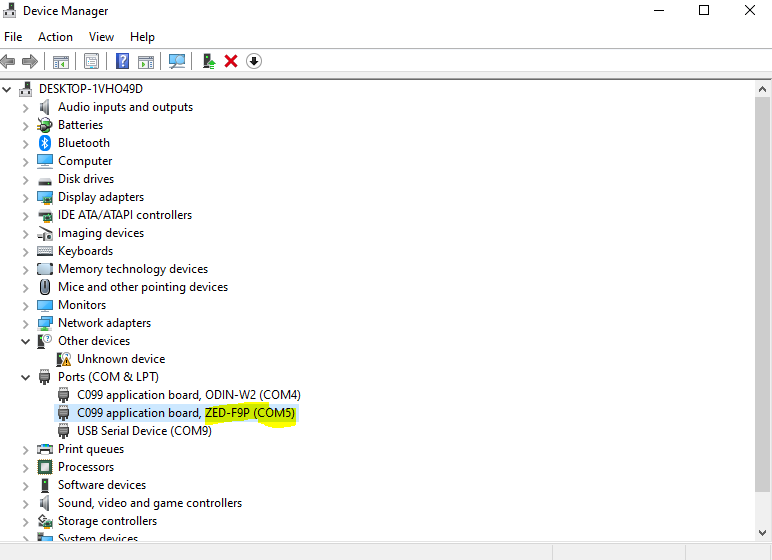
\includegraphics[width=3in]{device_manager}. 
\end{center}

\subsection{The GUI is slow} 

Yes, that's because the laptop is slow and doesn't have enough memory. Sorry. I think I fixed all the crashes, but who knows! 


\section{Technical Data} 

\begin{itemize} 

\item GPS Receivers/Antennas/USB cables are from the ublox C099-F9P development board, which integrates the ZED-F9P dual-band GNSS receiver with an ODIN-W2 radio unit. More details about the board are available at \url{https://www.u-blox.com/en/product/c099-f9p-application-board}. 
\begin{itemize} 
\item The ``mbed" firmware is used for the ODIN-W2 radio unit, with the base configured as a WiFi AP and the rover as a WiFi station on the same network .

\end{itemize} 
\item Documentation/software/enclosure design are available at \url{https://github.com/cozzyd/c099-surveyer} 
\begin{itemize} 
\item STL files for the two parts of the 3-D printable enclosure are provided, as well as a FreeCAD project. 
\item Source code for the data logger is under \texttt{scripts/rover-gui}. 
\item Documentatio is available under the doc directory 
\end{itemize} 
\end{itemize} 




\end{document} 




